\documentclass[dvipdfmx,aspectratio=169]{beamer}
\usepackage{pxjahyper}							%しおりの文字化けを防ぐ
\renewcommand{\kanjifamilydefault}{\gtdefault}	%日本語フォントをゴシックに
\usepackage{graphics}							%各種画像の張り込み
\usepackage{amsmath,amssymb,mathtools}					%標準数式表現を拡大する
\usetheme[
	block=fill,
	progressbar=foot,
	numbering=fraction,
	subsectionpage=progressbar
]{Metropolis}
\usefonttheme{professionalfonts}

\usepackage{here}
\usepackage{booktabs}

\usepackage{tikz}
\usetikzlibrary{positioning}

\newcommand{\highlight}[2][yellow]{\tikz[baseline=(x.base)]{\node[rectangle,rounded corners,fill=#1!10](x){#2};}}
\newcommand{\highlightcap}[3][yellow]{\tikz[baseline=(x.base)]{\node[rectangle,rounded corners,fill=#1!10](x){#2} node[below of=x, color=#1]{#3};}}

\title{ディープラーニングの仕組みを知ろう!}
\subtitle{第0回 人工知能勉強会 準備編}
\author{Shion MORISHITA}
\institute{}
\date{\today}

\subject{\LaTeX{}+Beamer}
\begin{document}
	%タイトル
	\begin{frame}[plain]
	    \maketitle
	\end{frame}
	
	\begin{frame}{自己紹介}
		\alert{氏名}
		\begin{itemize}
			\item 森下 司温(MORISHITA Shion)
		\end{itemize}
		\alert{学校歴}
		\begin{itemize}
			\item 名城大学理工学部数学科
			\item 名古屋大学大学院情報学研究科複雑系科学専攻博士前期課程
		\end{itemize}
		\alert{趣味}
		\begin{itemize}
			\item 音楽(ピアノ、作編曲 など)
			\item ゲーム(Dead by Daylight、ぷよぷよ など)
			\item AI開発
		\end{itemize}
	\end{frame}
	
	\begin{frame}[shrink]{目次}
		\vspace{1em}
		\tableofcontents
	\end{frame}
	
	\section{はじめに}
	\begin{frame}{はじめに}
		\begin{block}{目的}
			\begin{itemize}
				\item 人工知能の現状について概要を知る
				\item ディープラーニングを理解するために必要な数学の概要を知る
			\end{itemize}
		\end{block}
	\end{frame}

	\section{人工知能の世界へようこそ}
	\subsection{人工知能とは?}
	\begin{frame}{人工知能(Artificial Intelligence; AI)とは?}
		\underline{「人工知能の定義」は確定していない}
		\begin{itemize}
			\item そもそも「知能」を、現代の人類は定義できていない
		\end{itemize}
		\underline{ジョン・マッカーシー氏\footnote{AI という語を最初に作った人}による定義}
		\begin{itemize}
			\item
				``the science and engineering of making intelligent machines, \\especially, intelligent computer programs''\\
				知的な機械、特に、知的なコンピュータプログラムを作る科学と工学
		\end{itemize}
	\end{frame}
	
	\subsection{AIの歴史}
	\begin{frame}[shrink]{AIの歴史}
		\begin{table}[h]
			\centering
			\begin{tabular}{lp{35em}p{40em}}
				\toprule
				\multicolumn{1}{c}{年代} & \multicolumn{1}{c}{概要} & \multicolumn{1}{c}{代表的な概念・技術} \\
				\midrule
				1950年~1960年            & \begin{minipage}{35em}
												\begin{itemize}
													\item アラン・チューリング氏が AI の起源となる概念を提唱
													\begin{itemize}
														\item 機械は考えることができるのか?
													\end{itemize}
													\item ジョン・マッカーシー氏が「知的な機械、特に、知的なコンピュータプログラムを作る科学と工学」として人工知能を定義
												\end{itemize}
											\end{minipage} & \begin{minipage}{40em}
												\begin{itemize}
													\item \alert{チューリングテスト}
													\begin{itemize}
														\item 機械が思考したかどうかは、人との会話が成立したかどうかで判断
													\end{itemize}
												\end{itemize}
											\end{minipage} \\
				\midrule
				1960年~1974年            & \begin{minipage}{35em}
												\begin{itemize}
													\item 第1次AIブーム到来
													\item 対話できる自然言語プログラム「\alert{イライザ}(ELIZA)」が誕生
												\end{itemize}
											\end{minipage}
										& \begin{minipage}{40em}
											\begin{itemize}
												\item コンピュータの\alert{推論}・\alert{探索}
												\begin{itemize}
													\item 推論:人間が施行する過程を記号で表現し、実行すること
													\item 探索:目的となる条件を、解き方のパターンを場合分けして探し出していくこと
												\end{itemize}
												\item \alert{イライザ}(ELIZA)
												\begin{itemize}
													\item 特定のキーワードに反応する回答パターンを複数持たせたもの
													\item Siri の起源
												\end{itemize}
											\end{itemize}
										\end{minipage} \\
				\midrule
				1974年~1980年            & \begin{minipage}{35em}
												\begin{itemize}
													\item ブームが下火に
													\begin{itemize}
														\item AIの性能が科学者間で疑問視
														\begin{itemize}
															\item 迷路の解き方といった簡単な課題にしか対応できなかった
															\item 現代社会でみられる、複数の要因が絡み合う課題は解けなかった
														\end{itemize}
													\end{itemize}
												\end{itemize}
											\end{minipage} & \\
				\midrule
				1980年~1987年            & \begin{minipage}{35em}
												\begin{itemize}
													\item 第2次AIブーム到来
													\item 「\alert{エキスパートシステム}」が事業に広く導入開始
													\item 後にディープラーニングの基礎となる「\alert{誤差逆伝播法}」が発表
												\end{itemize}
											\end{minipage}  
										& \begin{minipage}{40em}
											\begin{itemize}
												\item \alert{エキスパートシステム}
												\begin{itemize}
													\item 大量の知識ベース(もし~ならば...)を蓄積し、それを用いて推論させるシステム
												\end{itemize}
												\item \alert{誤差逆伝播法}
												\begin{itemize}
													\item AIが学習を行なう具体的な手法
													\item 当時は複雑なモデルを扱わないことやコンピュータの性能不足により、あまり歓迎的ではなかった
												\end{itemize}
											\end{itemize}
										\end{minipage}\\
				\midrule
				1987年~1993年            & \begin{minipage}{35em}
												\begin{itemize}
													\item ブームが下火に
													\begin{itemize}
														\item エキスパートシステムの性能的な限界
													\end{itemize}
												\end{itemize}
											\end{minipage} & \\
				\midrule
				1993年~                 & \begin{minipage}{40em}
												\begin{itemize}
													\item 第3次AIブーム到来
													\item \alert{機械学習}を応用した技術の実用化
													\item \alert{ビッグデータ}によるデータ蓄積の加速化
													\item 産業への\alert{ディープラーニング}の導入
												\end{itemize}
											\end{minipage}                                
										& \begin{minipage}{35em}
											\begin{itemize}
												\item \alert{機械学習}
												\item \alert{ビッグデータ}
												\item \alert{ディープラーニング}(2006年)
											\end{itemize}
										\end{minipage}\\
				\bottomrule                                                                                                      
			\end{tabular}
		\end{table}
	\end{frame}
	
	\subsection{AIの分類}
	\begin{frame}{課題処理の観点から分類}
		\begin{itemize}
			\item \alert{特化型AI}(Artificial Narrow Intelligence; ANI)
			\begin{itemize}
				\item 特定の狭い範囲の課題に対応したAI
				\item 現時点で登場しているすべてのAIはここに分類
			\end{itemize}
			\item \alert{汎用型AI}(Artificial General Intelligence; AGI)
			\begin{itemize}
				\item 人間のように広範囲の課題に対応したAI
				\item 現時点(\today)では実現されていない
			\end{itemize}
		\end{itemize}		
	\end{frame}
	\begin{frame}{分析技術の観点から分類(特化型AI)}
		\begin{itemize}
			\item \alert{ルールベース}$ = $大量の知識ベース(もし~ならば...)を蓄積し、それをもとに推論するシステム
			\item \alert{機械学習}$ = $コンピュータに大量のデータを学習させ、分類や予測などを行なうためのアルゴリズムやモデルを構築する技術
			\begin{itemize}
				\item \alert{教師あり学習}
				\begin{itemize}
					\item 入力データ(問題)と教師データ(模範解答)を用いて、入力に対して正しい出力が得られるよう、自動で学習
					\item 未知の入力データ(問題)に対しても適切な出力データ(回答)が取得可能
				\end{itemize}
				\item \alert{教師なし学習}
				\begin{itemize}
					\item 入力データのみを用いて自動的に学習
					\item データの構造やパターンを発見可能
				\end{itemize}
				\item \alert{強化学習}
				\begin{itemize}
					\item 環境との相互作用を通じて、最適な行動を自動的に学習
				\end{itemize}
			\end{itemize}
		\end{itemize}
	\end{frame}
	
	\subsection{ディープラーニング}
	\begin{frame}{ディープラーニングとは}
		\begin{itemize}
			\item 教師あり学習に分類される、機械学習の一手法
			\item 大量のデータを使って、コンピュータが自動的に特徴を学習
			\item 画像認識、音声認識、自然言語処理など、さまざまな分野で活用可能
		\end{itemize}
	\end{frame}
	
	\begin{frame}{解決しうる問題の大前提}
		\begin{itemize}
			\item 人間側のある入力に対して、適切と思われるAI側の出力が欲しい
			\begin{itemize}
				\item \underline{顔認証システム}\\(入力:顔の画像/出力:本人かどうかの YES or NO)
				\item \underline{自動字幕システム}\\(入力:声/出力:喋った文章)
				\item \underline{ChatGPT}\\(入力:質問/出力:回答)
				\item \underline{競馬で3着以内に入る馬の予測}\\(入力:馬情報や当日レース情報、同馬の過去レース情報など/出力:3着以内に入りそうな馬の一覧)
			\end{itemize}
		\end{itemize}
	\end{frame}
	
	\begin{frame}{ディープラーニングの仕組み(概要)}
		\begin{itemize}
			\item \alert{ニューラルネットワーク}($ \simeq $脳)を用いて学習
			\begin{itemize}
				\item \alert{入力データ}
				\begin{itemize}
					\item 感覚器官からの刺激
				\end{itemize}
				\item \alert{ニューラルネットワーク}
				\begin{itemize}
					\item 脳の神経細胞の集まり
				\end{itemize}
				\item \alert{出力データ}
				\begin{itemize}
					\item 行動や反応
				\end{itemize}
			\end{itemize}
			\item
				実際に行った行動や反応(\alert{出力データ})と、本来取るべきだった行動や反応(\alert{正解データ})を比べて、\underline{そのズレがなくなるように}ニュラルネットワークをアップデートすることを繰り返す
		\end{itemize}
	\end{frame}

	\begin{frame}{ディープラーニングの仕組み(概要)}
		% TODO: \usepackage{graphicx} required
		\begin{figure}
			\centering
			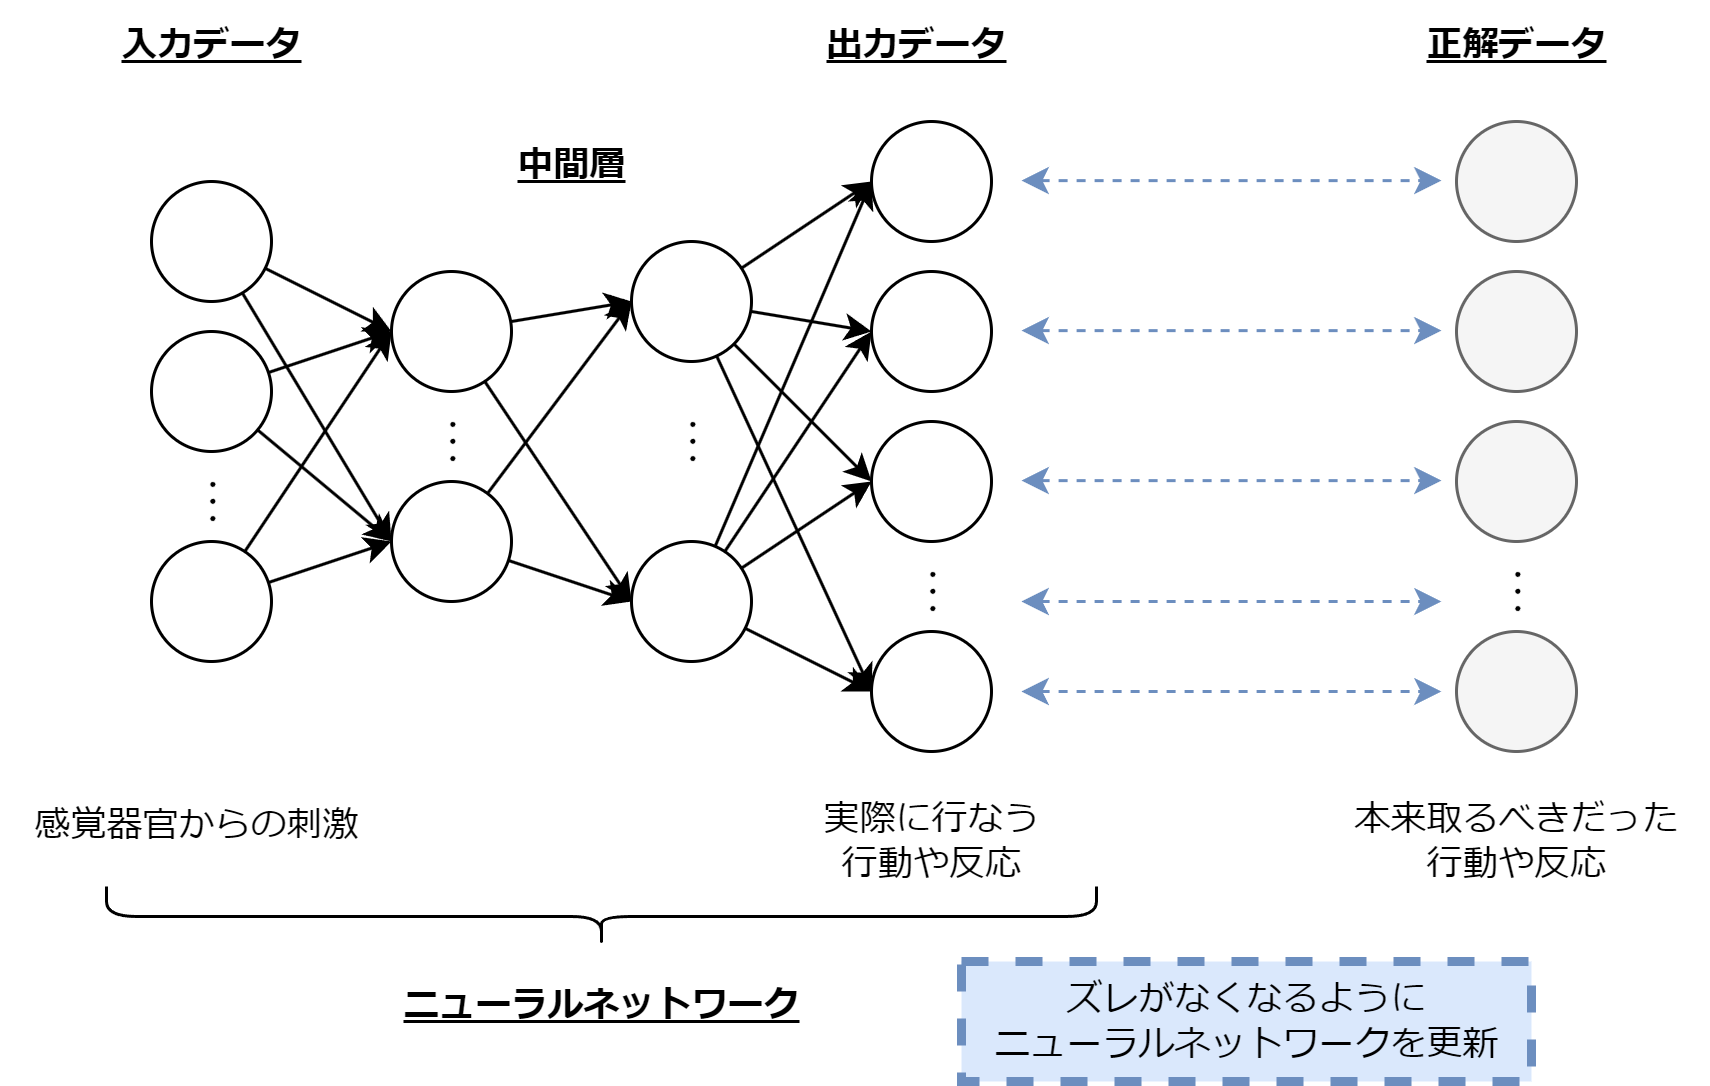
\includegraphics[width=0.8\linewidth]{img/how-deep-learning-works(overview)}
		\end{figure}
	\end{frame}

	\begin{frame}{ディープラーニングに必要な数学の最短ロードマップ}
		\begin{figure}
			\centering
			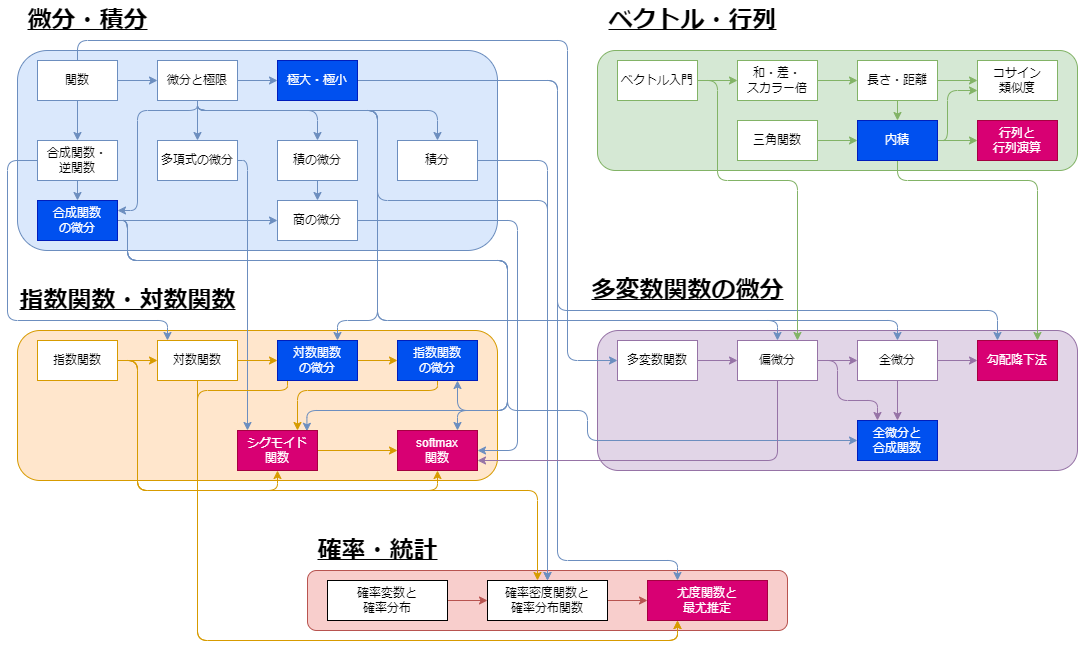
\includegraphics[width=0.85\linewidth]{img/math-roadmap}
		\end{figure}
	\end{frame}
	
	\section{現状の理解度チェック}
	\begin{frame}{現状の理解度チェック:$ \displaystyle\sum $}
		高度な大学数学は扱いません。
		
		ほとんどが高校数学か、その延長です。
		
		足りない知識はその都度確認を入れるので、\\まずは現状の理解度をチェックしましょう!
		
		\hrulefill
		
		\begin{itemize}
			\item[□]
				$ \displaystyle\sum $の意味は分かるか?(数B)
				\begin{itemize}
					\item
					$ \displaystyle\sum_{k=1}^n x_k = x_1 + x_2 + \dots + x_n. $
				\end{itemize}
		\end{itemize}
	\end{frame}
	\begin{frame}{現状の理解度チェック:ベクトル}
		\begin{itemize}
			\item[□]
				ベクトルを知っているか?(数B)
				\begin{itemize}
					\item
						高校数学の場合:$ \overrightarrow{a} = (1,2,3) $(行ベクトル)
					\item
						大学数学の場合:$ \boldsymbol{a} = \begin{bmatrix}
							1\\ 2\\ 3
						\end{bmatrix} $(列ベクトル)
				\end{itemize}
			\item[□]
				ベクトルの加法や内積の計算ができるか?(数B)
				\begin{itemize}
					\item
						$ \begin{bmatrix}
							\highlight[red]{1}\\ \highlight[red]{2}\\ \highlight[red]{3}
						\end{bmatrix} + \begin{bmatrix}
							\highlight[blue]{-2}\\ \highlight[blue]{3}\\ \highlight[blue]{-5}
						\end{bmatrix} = \begin{bmatrix}
							\highlight[red]{1}&+&\highlight[blue]{(-2)}\\ \highlight[red]{2}&+&\highlight[blue]{3}\\ \highlight[red]{3}&+&\highlight[blue]{(-5)}
						\end{bmatrix} = \begin{bmatrix}
							-1\\ 5\\ -2
						\end{bmatrix}. $
					\item
						$ \left\langle \begin{bmatrix}
							\highlight[red]1\\ \highlight[red]2\\ \highlight[red]3
						\end{bmatrix}, \begin{bmatrix}
						\highlight[blue]{-2}\\ \highlight[blue]3\\ \highlight[blue]{-5}
					\end{bmatrix} \right\rangle = \highlight[red]1 \cdot \highlight[blue]{(-2)} + \highlight[red]2 \cdot \highlight[blue]3 + \highlight[red]3 \cdot \highlight[blue]{(-5)} = -11. $
				\end{itemize}
		\end{itemize}
	\end{frame}
	\begin{frame}{現状の理解度チェック:行列}
		\begin{itemize}
			\item[□]
				行列を知っているか?(大学数学)
				\begin{itemize}
					\item
						$ \begin{bmatrix}
							1 & -1 & 0\\
							2 & 1 & -1\\
							-2 & 0 & 1
						\end{bmatrix} $
				\end{itemize}
			\item[□]
				行列とベクトルの積を知っているか、\\
				あるいは、下の式を理解できそうか?(大学数学)
				\begin{itemize}
					\item
						$ \begin{bmatrix}
							\highlight[red]{1} & \highlight[red]{-1} & \highlight[red]{0}\\
							\highlight[orange]{2} & \highlight[orange]{1} & \highlight[orange]{-1}\\
							\highlight[yellow]{-2} & \highlight[yellow]{0} & \highlight[yellow]{1}
						\end{bmatrix} \begin{bmatrix}
							\highlight[blue]{1}\\ \highlight[blue]{2}\\ \highlight[blue]{3}
						\end{bmatrix}  = \begin{bmatrix}
							\highlight[red]{1}\cdot\highlight[blue]{1} &+& \highlight[red]{(-1)}\cdot\highlight[blue]{2} &+& \highlight[red]{0}\cdot\highlight[blue]{3}\\
							\highlight[orange]{2}\cdot\highlight[blue]{1} &+& \highlight[orange]{1}\cdot\highlight[blue]{2} &+& \highlight[orange]{(-1)}\cdot\highlight[blue]{3}\\
							\highlight[yellow]{(-2)}\cdot\highlight[blue]{1} &+& \highlight[yellow]{0}\cdot\highlight[blue]{2} &+& \highlight[yellow]{1}\cdot\highlight[blue]{3}
						\end{bmatrix} = \begin{bmatrix}
							-1\\ 1\\ 1
						\end{bmatrix}$
				\end{itemize}
		\end{itemize}
	\end{frame}
	\begin{frame}{現状の理解度チェック:微分}
		\begin{itemize}
			\item[□]
				微分の計算は理解できるか?(数II)
				\begin{itemize}
					\item
					$ (e^x)' = \dfrac{\mathrm{d}}{\mathrm{d}x} e^x = e^x. $\vspace{0.2em}
					\item
					$ \dfrac{\mathrm{d}}{\mathrm{d}t} (t-1)^2 = 2(t-1). $
				\end{itemize}
			\item[□]
				合成関数の微分は知っているか?(数III)\\
				(今は忘れていても、下の式をなんとなく見た記憶があるか?)
				\begin{itemize}
					\item
					$ \dfrac{\mathrm{d}y}{\mathrm{d}x} = \dfrac{\mathrm{d}y}{\mathrm{d}u} \dfrac{\mathrm{d}u}{\mathrm{d}x} $(合成関数の微分の公式)
				\end{itemize}
		\end{itemize}
	\end{frame}
	\begin{frame}{現状の理解度チェック:多変数関数}
		\begin{itemize}
			\item[□]
				多変数関数を知っているか、\\
				あるいは、下の式を理解できるか?(大学数学)
				\begin{itemize}
					\item
						$ f(x, y) = x^2 + y^2 $のとき、$ f(1, 2) = 1^2 + 2^2 = 5. $
				\end{itemize}
			\item[□]
				偏微分の記号の意味を知っているか、\\
				あるいは、下の式を理解できるか?(大学数学)
				\begin{itemize}
					\item
						$ f(x,y) = x^2 + 2xy + y^2 $のとき、
						\begin{itemize}
							\item
								$ f_x(x,y) = \dfrac{\partial f}{\partial x} = 2x + 2y. $
							\item
								$ f_{xy}(x,y) = \dfrac{\partial}{\partial y} \left(\dfrac{\partial}{\partial x} f(x,y) \right) = \dfrac{\partial}{\partial y} (2x + 2y) = 2. $
						\end{itemize}
				\end{itemize}
		\end{itemize}
	\end{frame}	
\end{document}
